	\subsection{Taxonomy of virtualization by \textit{Ameen}}
	
	\begin{figure}[H]
		\centering
		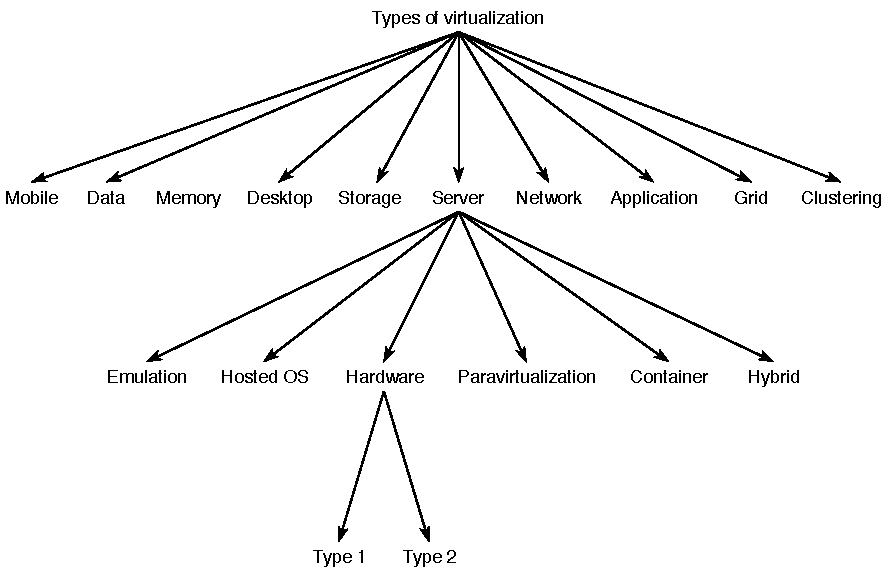
\includegraphics[width=8.5cm]{images/AmeenAndHamo2003.pdf}
		\caption{Taxonomy of virtualization by \textit{Ameen and A Hamo} \cite{Ameen2013}.} 
		\label{fig:TaxonomyOfVirtualizationByAmeen}
		%\vspace{1mm} 
	\end{figure}

%\noindent\rule{8.5cm}{0.4pt}
%		\vspace{1mm}
%	    \parbox[c]{8.5cm}{ \footnotesize Figure bases on the study \textit{A Survey of Server Virtualization} by Radhwan Y. Ameen and Asmaa Y. Hamo, in 2013}
%		\noindent\rule{8.5cm}{0.4pt}	    

%	\footnotetext [10]{Figure bases on the study \textit{A Survey of Server Virtualization} by Radhwan Y. Ameen and Asmaa Y. Hamo, in 2013.}

    From the perspective of the work of Ameen and Asmaa \cite{Ameen2013}, there are many different types of virtualization. In its first level is located some domains as  Mobile, Data, Memory, Desktop, Storage, Server, Network, Application, Grid and Clustering. Only Server virtualization is further decomposed. The second level shows the types considered for the Server Virtualization as Emulation, Hosted OS, Hardware, Paravirtualization, Container and Hybrid. Finally, the third level shows the types of virtualization considered for Hardware as Type 1 and Type 2. See Figure \ref{fig:TaxonomyOfVirtualizationByAmeen}.
    
    
    \textbf{Mobile virtualization} is a thin layer of software that is embedded on a mobile device to decouple the applications and data from the underlying hardware \cite{Ameen2013, VMware2018Website}. \textbf{Data virtualization} abstracts the source of individual data elements to allow applications to access data with a single methodology, regardless of how or where the data is stored \cite{Mann2006}. \textbf{Memory virtualization} consists of adding an extra level of address translation to give each VM the illusion of having zero memory address space, as provided by real hardware \cite{Ameen2013, Waldspurger2002}. \textbf{Desktop virtualization} is described as the ability to display a graphical desktop from one computer system on another computer system or device \cite{Ameen2013, VonHagen2008}. \textbf{Storage virtualization} is the emerging technology that creates logical abstractions of physical storage systems \cite{Ameen2013, Bigang2005}. \textbf{Server virtualization} is defined as the ability to run many operating systems with isolation and independence on other operating system \cite{Ameen2013}.
    \textbf{Network virtualization} provides an abstraction layer that can decouple the physical network equipment from the delivered business services over the network \cite{Annapareddy2011}. \textbf{Application virtualization} allows the user to run the application using local resources without installing the application in his system completely \cite{Annapareddy2011}. It also provides smaller single application virtual machines that allow for emulation of a specific environment on a client system.\cite{White2010}. \textbf{Grid virtualization} provides a way to abstract multiple physical servers (generally heterogeneous) from the application they are running \cite{Mann2006}. In \textbf{Clustering virtualization}, a cluster makes several locally-attached physical systems appear to the application and end users as a single processing resource \cite{Ameen2013, Mann2006}.
    
    Under the Server virtualization category,  \textbf{Emulation} is a virtualization method in which a complete hardware architecture may be created in software. This software is able to replicate the functionality of a designated hardware processor and associated hardware systems. \cite{Mann2006, Chiueh2005, VonHagen2008}.    \textbf{Hosted OS} virtualization is a software-only approach using a hypervisor layer that is hosted in an underlying operating system \cite{Ameen2013, VonHagen2008}. \textbf{Hardware} virtualization  is also referred to as hardware-assisted or full virtualization. Here the hypervisor is assisted by the processor hardware such as AMD-V or Intel VT-x processor virtualization technologies \cite{Ameen2013, VonHagen2008}. Hardware virtualization is further decomposed into  Type 1 and Type 2 hypervisors as we have seen in other classifications. 

    
    \textbf{Paravirtualization} refers to a technique in which the guest OS includes modified (paravirtualized) I/O drivers for the hardware. Unlike a binary translation approach, the hypervisor does not need to trap and translate all privileged layer instructions between the guest OS and the actual server hardware. Instead, the modified guest OS makes calls directly to the virtualized I/O services and other privileged operations \cite{Ameen2013, VonHagen2008}. \textbf{Container} virtualization is a kernel-layer abstraction and refers to  techniques in which the abstraction technology is built directly into the OS kernel rather than having a separate hypervisor layer \cite{Ameen2013, Lin2012}. Amen and Asmaa also includ the category \textbf{Hybrid}, referring to a combination of full virtualization and paravirtualization that uses input/output (I/O) acceleration techniques \cite{Ameen2013, White2010}.

    
    
    The Ammen and Asmaa's study is closely related to the works of Kampert \cite{Kampert2010} and Kusnetzky \cite{Kusnetzky2011} and presents a classification scheme through a three-level hierarchical structure. Although this graphical representation is simple and interesting, it is unbalanced because it focuses only on detailing the Server Virtualization category.



